%%%%%%%%%%%%%%%%%%%%%%%%%%%%%%%%%%%%%%%%%%%%%%%%%%%%%%%%%%%%%%%%%%%%%%%%%%%%%% 
\newpage
\section {Parameterization of the SINDRUM-II detector response}

%%%%%%%%%%%%%%%%%%%%%%%%%%%%%%%%%%%%%%%%%%%%%%%%%%%%%%%%%%%%%%%%%%%%%%%%%%%%%%
\subsection{Momentum Resolution}

Figure ~\ref{fig:dio_1} overlays the electron momentum spectrum measured by SINDRUM-II
and shifted by 0.5 MeV DIO spectrum on \Pb{208} calculated in \cite{Watanabe_1993}.
it is clear, that the two spectra have quite different slopes.
The sign of the difference is easy to understand as in case of a rapidly falling
spectrum, the finite experimental resolution smears the spectrum and effectively
reduces the observed slope. 

\vspace{0.2in}
\begin{tikzpicture}
  \node[anchor=south west,inner sep=0] at (0,0.) {
    % \node[shift={(0 cm,0.cm)},inner sep=0,rotate={90}] at (0,0) {}
    \makebox[\textwidth][c] {
      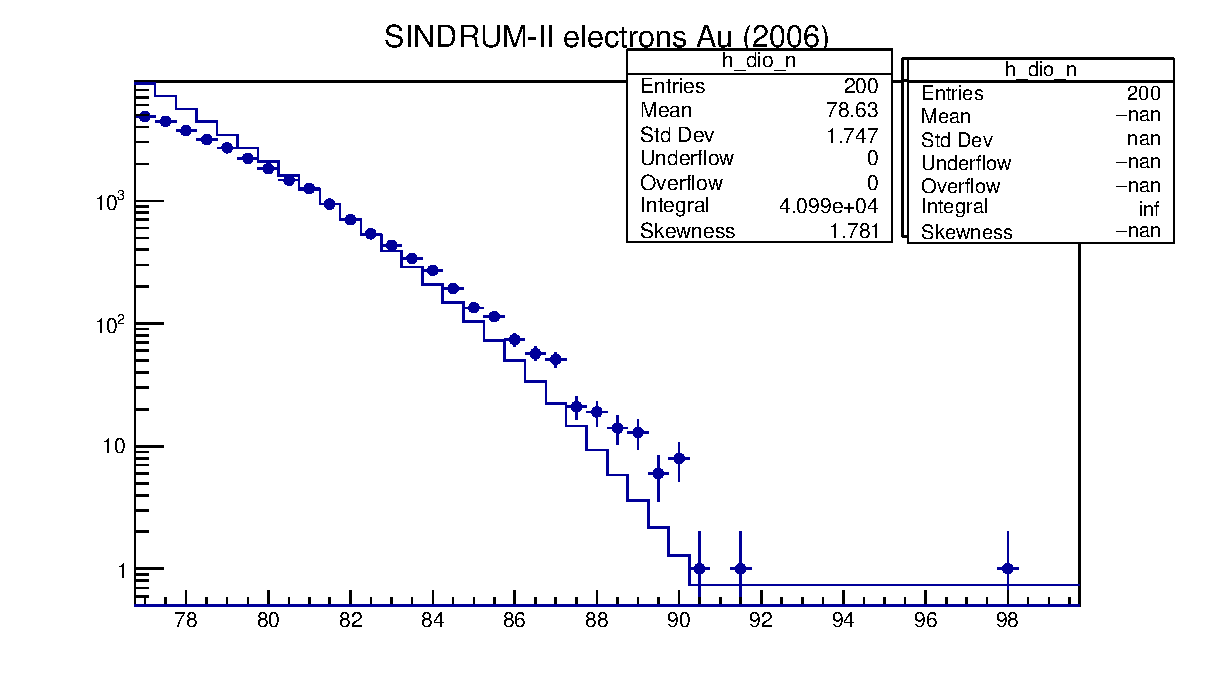
\includegraphics[width=1.0\textwidth]{figures/png/ana_step1_dio_normalized_above_80}
    }
  };
  % \node [text width=6cm, scale=0.8] at (4.5,6.4) {mu2e-18894 by Kevin Lynch and Jim Popp};
\end{tikzpicture}
\captionof{figure} {
  \label{fig:dio_1}
  SINDRUM-II electron spectrum overlayed with the DIO spectrum from \cite{Watanabe_1993}.
  The two spectra are normalized to the same area for p > 80 MeV/c
}

\vspace{0.2in}
We make a [simplified] assumption that the detector momentum resolution response
is symmetric and can be described by a single gaussian function. 
The experimental momentum resolution is one of the parameters of the detector response model.
To choose the optimal value, we vary the resolution in the range [1, 3.5] MeV/c, convolute the
theoretical DIO spectrum with the given resolution, and use the resulting distribution to fit
the SINDRUM-II electron spectrum. Fit has one parameter - normalization. Fit chi2 dependence
on the $\sigma_P$ is shown in Figure ~\ref{fig:ana_step1_fit_sigma}, the best value of the resolution
parameter is $\sigma_P = 2.0 \pm 0.1$ MeV/c. This value is significantly higher than the momentum
resolution of the SINDRUM-II detector and is likely due to that contribution of RMC electrons
not accounted for in the procedure. As one can see from Figure ~\ref{fig:sindrum_ii_2006_fig_11},
for momenta close to 90 MeV/c, contribution of RMC could be non-negligible. As the RMC spectrum
is less steep than the DIO one, ignoring RMC contribution should result in larger value of the
best resolution parameter returned by the procedure described above.

\vspace{0.2in}
\begin{tikzpicture}
  \node[anchor=south west,inner sep=0] at (0,0.) {
    % \node[shift={(0 cm,0.cm)},inner sep=0,rotate={90}] at (0,0) {}
    \makebox[\textwidth][c] {
      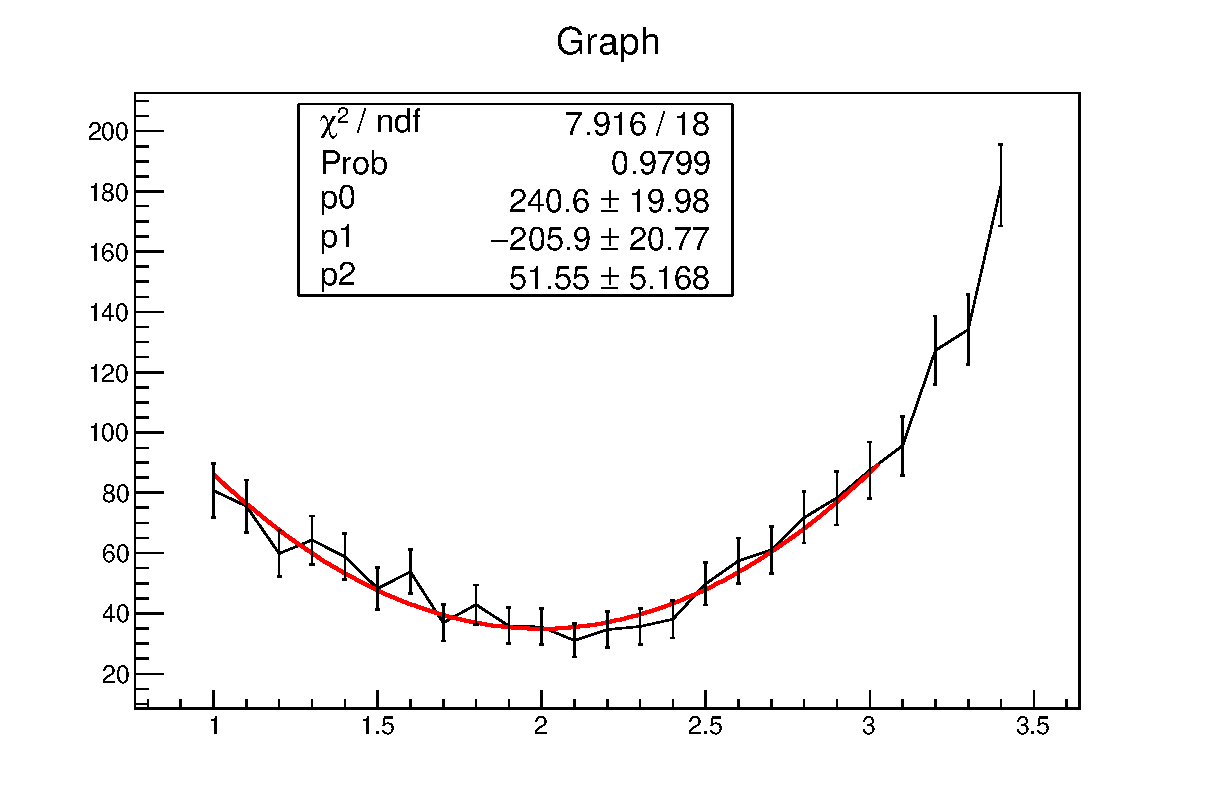
\includegraphics[width=0.9\textwidth]{figures/png/ana_step1_fit_sigma}
    }
  };
  % \node [text width=6cm, scale=0.8] at (4.5,6.4) {mu2e-18894 by Kevin Lynch and Jim Popp};
\end{tikzpicture}
%
\captionof{figure} {
  \label{fig:ana_step1_fit_sigma}
  chi2 of the fit of the SINDRUM-II DIO electron spectrum with the theoretical distribution
  convoluted with a gaussian with given resolution $\sigma_P$ as a function of $\sigma_P$.
}
\vspace{0.2in}

%%%%%%%%%%%%%%%%%%%%%%%%%%%%%%%%%%%%%%%%%%%%%%%%%%%%%%%%%%%%%%%%%%%%%%%%%%%%%%
\subsection{Tracking Efficiency}

To parameterize the SINDRUM-II tracking efficiency, we assume that it is flat
above 80 MeV/c. Normalizing the DIO spectrum convoluted with $\sigma_P = 2.0$ MeV/c
resolution to the electron data in the region p > 80 MeV and dividing the data spectrum
by the resulting distribution gives the ``efficiency'' dependence on the track momentum
shown in Figure ~\ref{fig:ana_step1_efficiency}

Assume efficiency flat above 80 MeV/c, normalize MC to data in that region:

\begin{tikzpicture}
  \node[anchor=south west,inner sep=0] at (0,0.) {
    % \node[shift={(0 cm,0.cm)},inner sep=0,rotate={90}] at (0,0) {}
    \makebox[\textwidth][c] {
      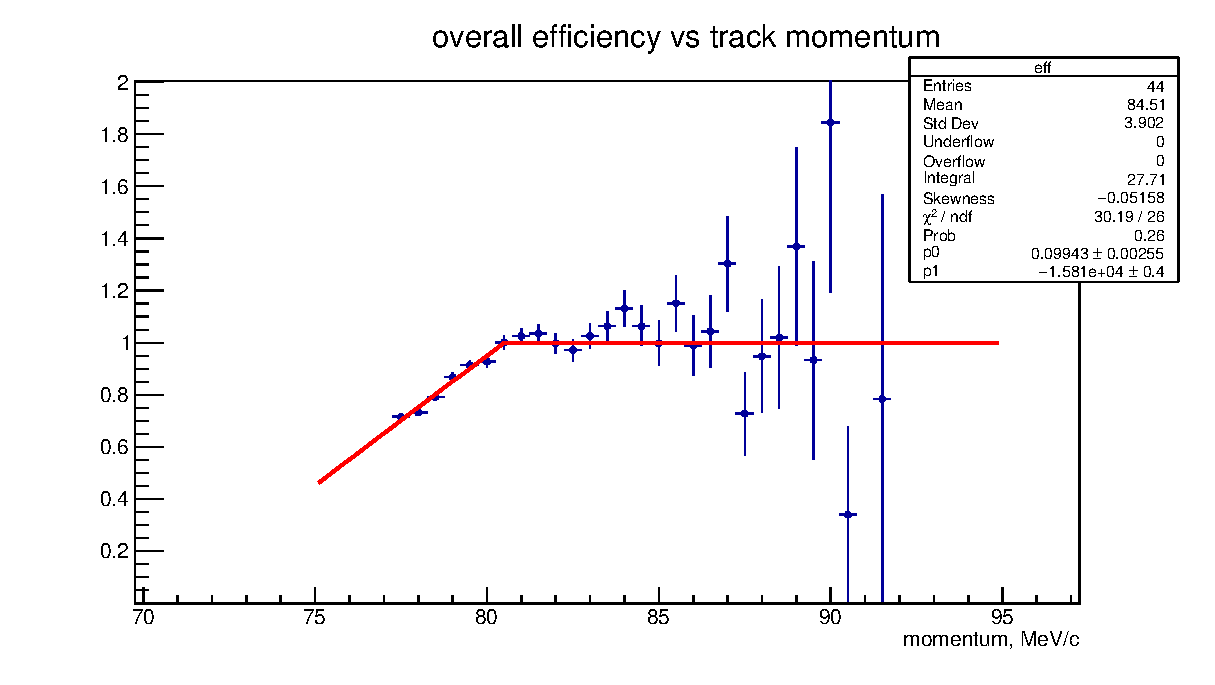
\includegraphics[width=0.9\textwidth]{figures/png/ana_step1_efficiency}
    }
  };
  % \node [text width=6cm, scale=0.8] at (4.5,6.4) {mu2e-18894 by Kevin Lynch and Jim Popp};
\end{tikzpicture}
%
\captionof{figure} {
  \label{fig:ana_step1_efficiency}
  Parameterization of the SINDRUM-II efficiency vs the track momentum.
  Definition of efficiency includes all components - trigger, reconstruction and selection.
  Overall normalization is chosen such that efficiency is equal to one for p > 80 MeV/c
}
\vspace{0.2in}

This step concludes tuning of the detector response, Figure \ref{fig:ana_step1_best_dio_fit}.
shows description of the electron spectrum with the tuned response.

\vspace{0.2in}
\begin{tikzpicture}
  \node[anchor=south west,inner sep=0] at (0,0.) {
    % \node[shift={(0 cm,0.cm)},inner sep=0,rotate={90}] at (0,0) {}
    \makebox[\textwidth][c] {
      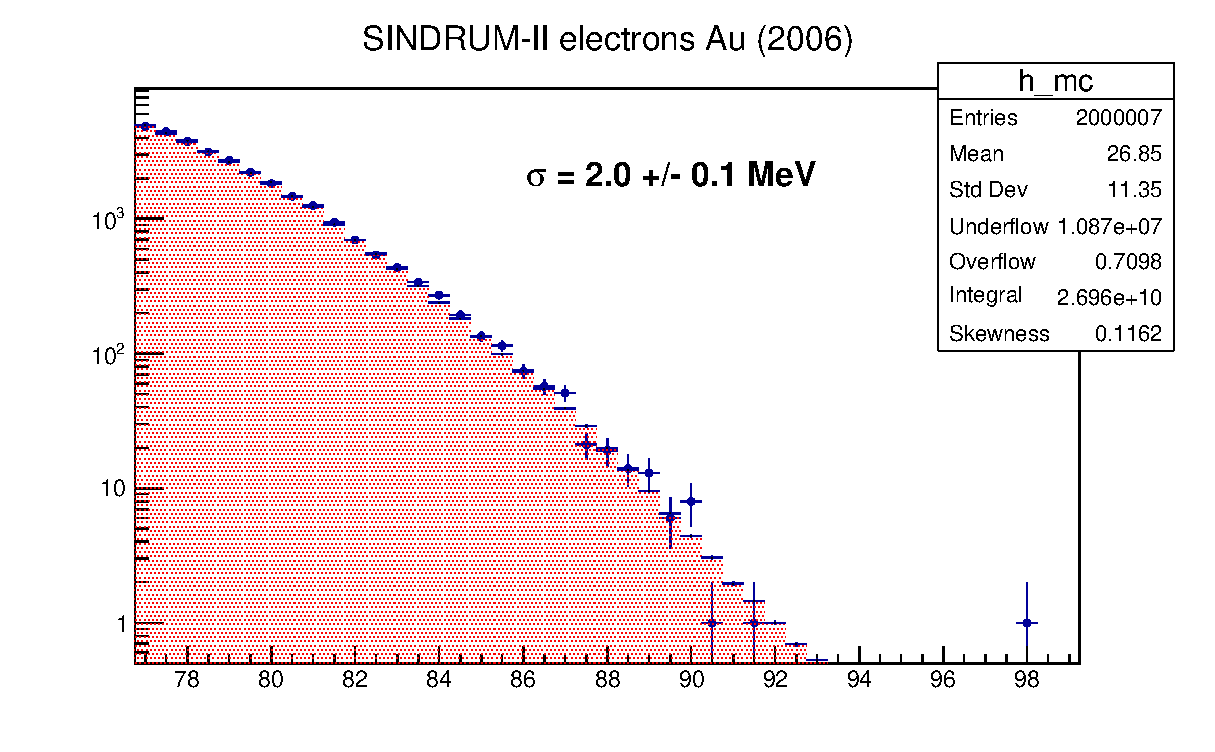
\includegraphics[width=0.99\textwidth]{figures/png/ana_step1_best_dio_fit}
    }
  };
  % \node [text width=6cm, scale=0.8] at (4.5,6.4) {mu2e-18894 by Kevin Lynch and Jim Popp};
\end{tikzpicture}
%
\captionof{figure} {
  \label{fig:ana_step1_best_dio_fit}
  Description of the electron spectrum on Au target from \cite{sindrum_ii:Bertl2006}
  with the tuned model of the SINDRUM-II detector response.
}
